\documentclass{beamer}

\usetheme{CambridgeUS}
\usecolortheme{orchid}

\usepackage{wrapfig}
\usepackage{siunitx}
\usepackage{pgfplots}
\usepackage{inconsolata}
\usepackage{amsmath}
\usepackage{bm}
\usepackage{nicefrac}
\usepackage{tikz}
\usetikzlibrary{shapes.geometric, positioning, automata, shapes, arrows, calc}

\definecolor{darkblue}{HTML}{00688B}
\definecolor{darkgreen}{HTML}{6E8B3D}
\definecolor{cadet}{HTML}{DAE1FF}
\definecolor{salmon}{HTML}{FFB08A}

\newcount\gaussF
\edef\gaussR{0}
\edef\gaussA{0}

\makeatletter
\pgfmathdeclarefunction{gaussR}{0}{%
 \global\advance\gaussF by 1\relax
 \ifodd\gaussF
  \pgfmathrnd@%
  \ifdim\pgfmathresult pt=0.0pt\relax%
    \def\pgfmathresult{0.00001}%
  \fi
  \pgfmathln@{\pgfmathresult}%
  \pgfmathmultiply@{-2}{\pgfmathresult}%
  \pgfmathsqrt@{\pgfmathresult}%
  \global\let\gaussR=\pgfmathresult%radius
  \pgfmathrnd@%
  \pgfmathmultiply@{360}{\pgfmathresult}%
  \global\let\gaussA=\pgfmathresult%angle
  \pgfmathcos@{\pgfmathresult}%
  \pgfmathmultiply@{\pgfmathresult}{\gaussR}%
 \else
  \pgfmathsin@{\gaussA}%
  \pgfmathmultiply@{\gaussR}{\pgfmathresult}%
 \fi
}

\pgfmathdeclarefunction{invgauss}{2}{%
  \pgfmathln{#1}% <- might need parsing
  \pgfmathmultiply@{\pgfmathresult}{-2}%
  \pgfmathsqrt@{\pgfmathresult}%
  \let\@radius=\pgfmathresult%
  \pgfmathmultiply{6.28318531}{#2}% <- might need parsing
  \pgfmathdeg@{\pgfmathresult}%
  \pgfmathcos@{\pgfmathresult}%
  \pgfmathmultiply@{\pgfmathresult}{\@radius}%
}

\pgfmathdeclarefunction{randnormal}{0}{%
  \pgfmathrnd@
  \ifdim\pgfmathresult pt=0.0pt\relax%
    \def\pgfmathresult{0.00001}%
  \fi%
  \let\@tmp=\pgfmathresult%
  \pgfmathrnd@%
  \ifdim\pgfmathresult pt=0.0pt\relax%
    \def\pgfmathresult{0.00001}%
  \fi
  \pgfmathinvgauss@{\pgfmathresult}{\@tmp}%
}

\begin{document}

\title[ROM and POD]{
  A step towards Reduced Order Modelling of flow characterized by wakes using
  Proper Orthogonal Decomposition
}
\author[E. Fonn]{
  E.~Fonn\inst{1,2} \and
  A.~Rasheed\inst{2} \and
  M.~Tabib\inst{2} \and
  S.~Siddiqui\inst{2,3} \and
  T.~Kvamsdal\inst{3}
}
\institute[SINTEF]{
  \inst{1}%
  \url{eivind.fonn@sintef.no}
  \and \inst{2}%
  Applied Mathematics, SINTEF ICT
  \and \inst{3}%
  Department of Mathematical Sciences, NTNU
}
\date[OMAE 2017]{}

\titlegraphic{\includegraphics[width=0.3\textwidth]{sintef}}

\begin{frame}
  \titlepage{}
\end{frame}

\section{Background}

\begin{frame}[fragile]
  \frametitle{Background}

  High fidelity flow simulations are expensive.

  \begin{itemize}
  \item Millions or billions of degrees of freedom,
  \item days of computational time,
  \item require powerful parallel architectures.
  \end{itemize}

  These are surmountable challenges in many situations, but not all.
\end{frame}

\begin{frame}[fragile]
  \frametitle{Background}

  Many applications (e.g. optimization) require repetitive solution of PDEs.

  \begin{center}
    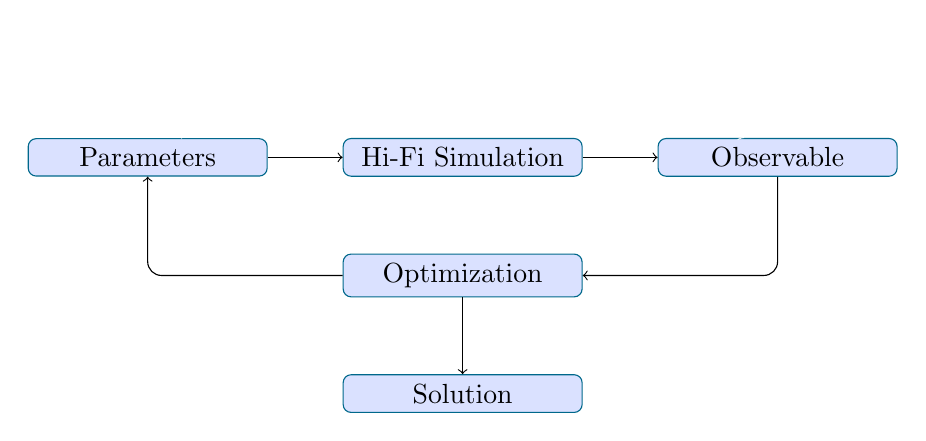
\begin{tikzpicture}[
      block/.style={
        minimum width=30mm,
        text width=28mm,
        align=center,
        rounded corners=1mm,
        draw=darkblue,
        fill=cadet,
      },
      ]
      \node[block] (param) at (-4,0) {Parameters};
      \node[block] (hifi) at (0,0) {Hi-Fi Simulation};
      \node[block] (obj) at (4,0) {Observable};
      \node[block] (opt) at (0,-1.5) {Optimization};
      \node[block] (sol) at (0,-3) {Solution};
      \draw[->] (param) edge (hifi);
      \draw[->] (hifi) edge (obj);
      \draw[->,rounded corners=5pt] (obj) |- (opt);
      \draw[->,rounded corners=5pt] (opt) -| (param);
      \draw[->] (opt) edge (sol);
      \draw[dashed,white,->] (param) edge[bend left] (obj);
    \end{tikzpicture}
  \end{center}
\end{frame}

\begin{frame}[fragile]
  \frametitle{Background}

  Ideally: we want to ``cheat'' by avoiding the expensive simulation step.

  \begin{center}
    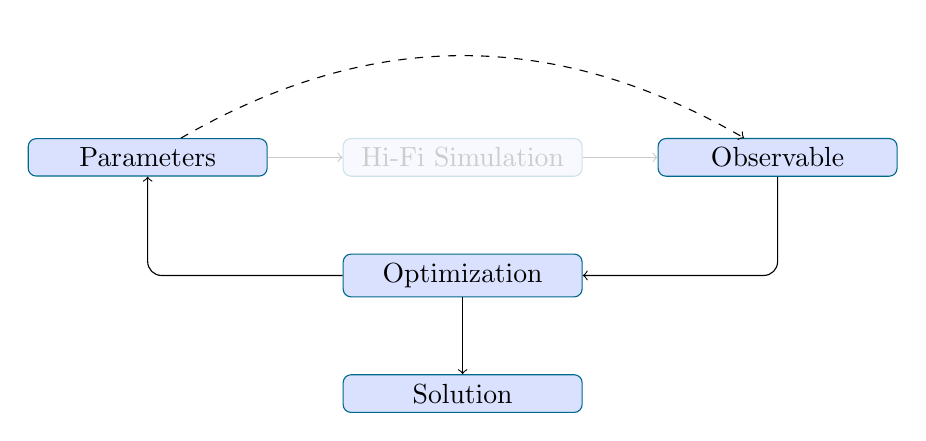
\begin{tikzpicture}[
      block/.style={
        minimum width=30mm,
        text width=28mm,
        align=center,
        rounded corners=1mm,
        draw=darkblue,
        fill=cadet,
      },
      ]
      \node[block] (param) at (-4,0) {Parameters};
      \node[block,draw=darkblue!20,fill=cadet!20,text=black!20] (hifi) at (0,0) {Hi-Fi Simulation};
      \node[block] (obj) at (4,0) {Observable};
      \node[block] (opt) at (0,-1.5) {Optimization};
      \node[block] (sol) at (0,-3) {Solution};
      \draw[->,black!20] (param) edge (hifi);
      \draw[->,black!20] (hifi) edge (obj);
      \draw[->,rounded corners=5pt] (obj) |- (opt);
      \draw[->,rounded corners=5pt] (opt) -| (param);
      \draw[->] (opt) edge (sol);
      \draw[dashed,->] (param) edge[bend left] (obj);
    \end{tikzpicture}
  \end{center}
\end{frame}

\section{Reduced bases}

\begin{frame}[fragile]
  \frametitle{Reduced bases}

  Idea: even though the solution space in a high-fidelity simulation has a very
  large number of DoFs, the space of ``typical'' solutions is
  \textbf{in practice} of considerably smaller dimension (several orders of
  magnitude). \\~\\

  Terms to be made more precise:
  \begin{itemize}
  \item ``typical''
  \item ``in practice''
  \end{itemize}

  ~\\

  In other words, we are paying for far greater variety in the solution space
  than we need.
\end{frame}

\begin{frame}[fragile]
  \frametitle{Reduced bases}

  We want to create a subspace of the larger solution space, where each basis
  function captures an ``essential feature'' of a typical solution. This basis
  is called a \textbf{reduced basis}. \\~\\

  Enter: Partial Orthogonal Decomposition, a.k.a. Principal Component Analysis.
  Can be thought of as an algorithm for
  \begin{itemize}
  \item dimensionality reduction, or
  \item low rank approximation, or
  \item feature extraction
  \end{itemize}
  or all of the above.
\end{frame}

\begin{frame}[fragile]
  \frametitle{Principal Components}

  \begin{center}
    \begin{tikzpicture}
      \foreach \i in {0,...,2000} {
        \fill [opacity=0.1,rotate=30] (randnormal, 0.3*randnormal) circle [radius=0.1];
      }
      \draw[->,rotate=30,red,very thick] (0,0) -- (1,0);
      \draw[->,rotate=30,red,very thick] (0,0) -- (0,1);
      \draw[->,green,very thick] (0,0) -- (1,0);
      \draw[->,green,very thick] (0,0) -- (0,1);
    \end{tikzpicture}
  \end{center}
\end{frame}

\begin{frame}[fragile]
  \frametitle{Partial Orthogonal Decomposition}

  \begin{itemize}
  \item Given: a set of parameter vectors $\bm\mu^i = (\mu^i_1, \ldots, \mu^i_P)$
  \item Compute: an ensemble of high-fidelity solutions $\varphi_i$
  \item Compute: the covariance matrix
    $C_{ij} = \left< \overline{\varphi}_i, \overline{\varphi}_j \right>_a$
  \item Compute: eigenpairs $(\lambda_m, \bm v^m)$ of $\bm C$
  \item Construct: modes $\zeta_m = \frac{1}{\sqrt{\lambda_m}} \sum_i v^m_i \varphi_i$
  \end{itemize}
\end{frame}

\begin{frame}[fragile]
  \frametitle{Partial Orthogonal Decomposition}

  \begin{itemize}
  \item The resulting modes $\zeta_m$ are orthonormal in the
    $\left< \cdot, \cdot \right>_a$ inner product.
  \item The eigenvalue $\lambda_m$ represents the amount of \emph{energy}
    captured by $\zeta_m$. Note:
    \[ \sum_m \lambda_m = \sum_i \| \varphi_i \|_a^2 \]
  \item Given a basis of the first $N$ modes, the tail of the eigenvalue sum
    represents the average \emph{approximation} error made.
    \[ \text{Avg.~rel.~error} = \sqrt{1 - \frac{\sum_{m=1}^N \lambda_m}{\sum_m \lambda_m}} \]
  \end{itemize}
\end{frame}

\begin{frame}[fragile]
  \frametitle{Terms}

  \begin{itemize}
  \item ``typical'': As understood by an implicit probability distribution over
    the parameter space. It is important that the ensemble of solutions is drawn
    from this probability distribution, and the resulting error estimate is to
    be regarded as the average error over that distribution.
  \item ``in practice'': The practical dimension of the solution space is the
    number of modes $N$ that reduces the error to a suitable
    application-dependent level.
  \end{itemize}
\end{frame}

\begin{frame}[fragile]
  \frametitle{The program}

  \begin{center}
    \begin{tikzpicture}[
      block/.style={
        minimum width=40mm,
        text width=38mm,
        align=center,
        rounded corners=1mm,
      },
      offline/.style={
        block,
        draw=darkblue,
        fill=cadet,
      },
      online/.style={
        block,
        draw=darkblue,
        fill=salmon,
      },
      clear/.style={
        block,
        draw=darkblue,
      },
      ]
      \node[offline] (pde) {\tiny Parametrized PDE};
      \node[offline, below=2mm of pde] (hifi) {
        \tiny
        High-fidelity discr. \\[0.5mm]
        $\bm A_h(\bm \mu) \bm u_h(\bm \mu) = \bm f_h(\bm \mu)$ \\[0.5mm]
        $\begin{aligned}
          \bm A_h &= \textstyle \sum_q \xi_q(\bm \mu) \bm A_h^q \\
          \bm f_h &= \textstyle \sum_q \chi_q(\bm \mu) \bm f_h^q
        \end{aligned}$
      };
      \node[offline, below=2mm of hifi] (snaps) {
        \tiny
        Generate a RB by applying POD to snapshot solutions, and construct
        projection matrix $\bm V$ \par
      };
      \node[offline, below=2mm of snaps] (proj) {
        \tiny
        Projection \\[1.0mm]
        $\begin{aligned}
          \bm A_N^q &= \bm V^\intercal A_h^q \bm V \\
          \bm f_N^q &= \bm V^\intercal f_h^q
        \end{aligned}$
      };
      \node[online, right=9mm of pde] (mu) {\tiny $\bm \mu$};
      \node[online, below=2mm of mu] (asm) {
        \tiny
        RB system assembly \\[1.0mm]
        $\begin{aligned}
          \bm A_N &= \textstyle \sum_q \xi_q(\bm \mu) \bm A_N^q \\
          \bm f_N &= \textstyle \sum_q \chi_q(\bm \mu) \bm f_N^q
        \end{aligned}$
      };
      \node[online, below=2mm of asm] (sol) {
        \tiny
        RB system solution \\[0.0mm]
        $\bm A_N(\mu) \bm u_N(\mu) = \bm f_N(\mu)$
      };
      \node[clear, below=2mm of sol] (err) {
        \tiny
        Error estimate \\[0.0mm]
        $\| \bm u_h(\mu) - \bm V \bm u_N(\mu) \|$
      };
      \node[clear, below=2mm of err] (rec) {
        \tiny
        Recovery, visualization and post-processing \\[0.0mm]
        $\bm u_N^h(\bm \mu) = \bm V \bm u_N(\bm \mu)$
      };
      \node[clear, below=2mm of rec] (eval) {
        \tiny
        Evaluating functionals of interest
      };

      \draw[->,rounded corners=5pt] (pde.south) -- (hifi.north);
      \draw[->,rounded corners=5pt] (hifi.south) -- (snaps.north);
      \draw[->,rounded corners=5pt] (snaps.south) -- (proj.north);
      \draw[->,rounded corners=5pt] (mu.south) -- (asm.north);
      \draw[->,rounded corners=5pt] (proj.east) -- ($(proj.east) + (3mm,0)$)
      -- ($(asm.west) - (6mm,0)$) -- (asm.west);
      \draw[->,rounded corners=5pt] (asm.south) -- (sol.north);
      \draw[->,rounded corners=5pt] (sol.west) -- ($(sol.west) - (3mm,0)$)
      -- ($(eval.west) - (3mm,0)$) -- (eval.west);
      \draw[->,rounded corners=5pt] ($(err.west) - (3mm,0)$) -- (err.west);
      \draw[->,rounded corners=5pt] ($(rec.west) - (3mm,0)$) -- (rec.west);
    \end{tikzpicture}
  \end{center}
\end{frame}

\section{Flow problems}

\begin{frame}[fragile]
  \frametitle{Flow problems}

  A Navier Stokes solver based on the PISO-SIMPLE (\emph{PIMPLE}) algorithm was
  used to provide snapshots for various problems.

  \begin{itemize}
  \item Flow around the cylinder
    \begin{itemize}
    \item constant and pulsating inflow conditions,
    \item $\text{Re}=256,2580,40000$
    \end{itemize}
  \item Flow around the NACA 0015 airfoil
    \begin{itemize}
    \item constant inflow conditions
    \item $\text{Re}=2\times\SI{e3}{},2\times\SI{e4}{},2\times\SI{e5}{}$
    \end{itemize}
  \end{itemize}

  Snapshots were sampled at a frequency of at least $20$ per principal period,
  and over at least $3$ periods.
\end{frame}

\begin{frame}[fragile]
  \frametitle{Flow problems}

  \begin{itemize}
  \item In the following, the first four modes and the first 200 elements of the
    energy spectra are shown.
  \item The covariance function has been chosen to be the velocity $L^2$ inner
    product, for the sake of simplicity. I.e.
    \[ \left< (\bm v_i, p_i), (\bm v_j, p_j) \right>_a
      = \int \bm v_i \cdot \bm v_j \]
  \item This means that modes are suitable to minimize the error in the velocity
    $L^2$ norm,
    \[ \| (\bm v, p) \|^2 = \int |\bm v|^2 \]
  \end{itemize}
\end{frame}

\begin{frame}[fragile]
  \frametitle{Cylinder, $\text{Re}=256$, first four modes}

  \begin{center}
    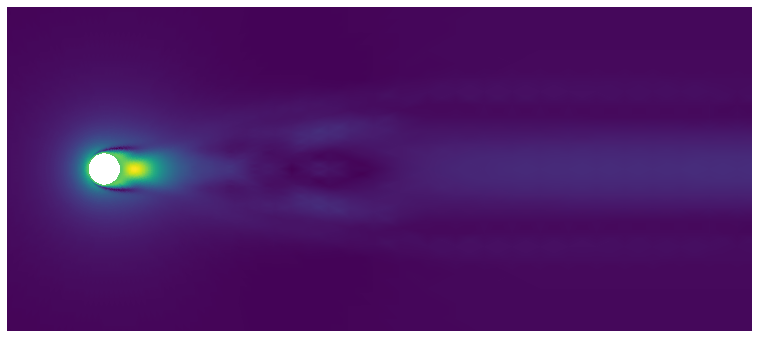
\includegraphics[width=0.49\textwidth]{figs/cyl_256_0}
    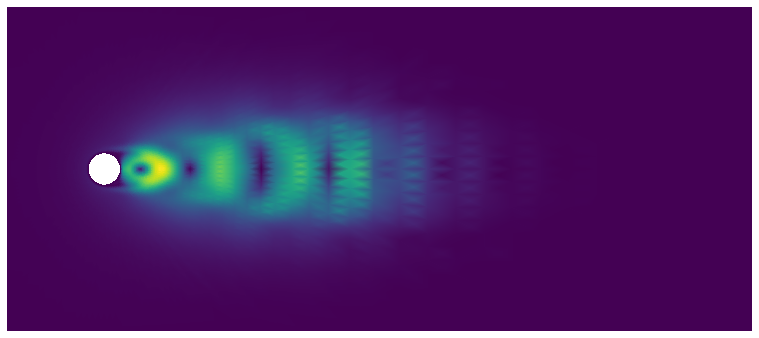
\includegraphics[width=0.49\textwidth]{figs/cyl_256_1} \\
    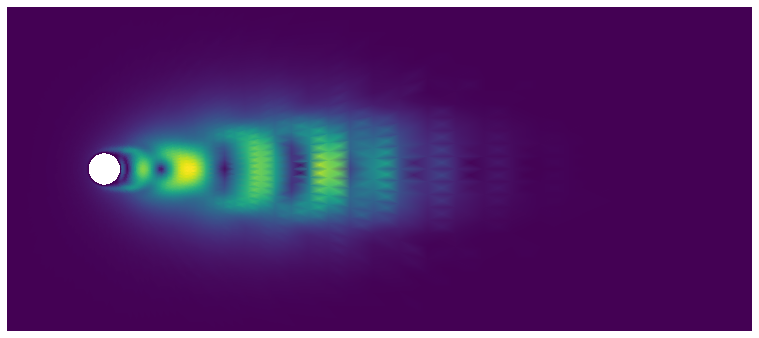
\includegraphics[width=0.49\textwidth]{figs/cyl_256_2}
    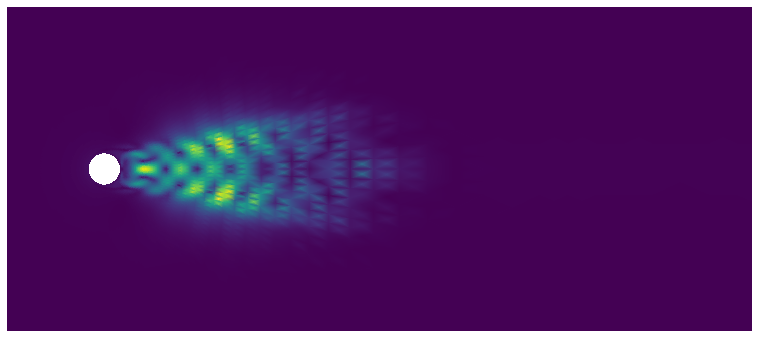
\includegraphics[width=0.49\textwidth]{figs/cyl_256_3}
  \end{center}
\end{frame}

\begin{frame}[fragile]
  \frametitle{Cylinder, $\text{Re}=256$, spectrum (normalized)}

  \begin{center}
    \begin{tikzpicture}
      \begin{axis}[
        ymode=log,
        grid=both,
        legend cell align=left,
        xmin=1, xmax=200,
        ]
        \addplot[magenta, very thick]
        table[x index={0}, y index={1}]{data/cyl_265.csv};
        \addplot[blue, very thick]
        table[x index={0}, y index={2}]{data/cyl_265.csv};
        \addplot[red, very thick]
        table[x index={0}, y index={3}]{data/cyl_265.csv};
        \legend{
          $\lambda_k$,
          Energy tail,
          Error,
        }
      \end{axis}
    \end{tikzpicture}
  \end{center}
\end{frame}

\begin{frame}[fragile]
  \frametitle{Cylinder, $\text{Re}=2580$, first four modes}

  \begin{center}
    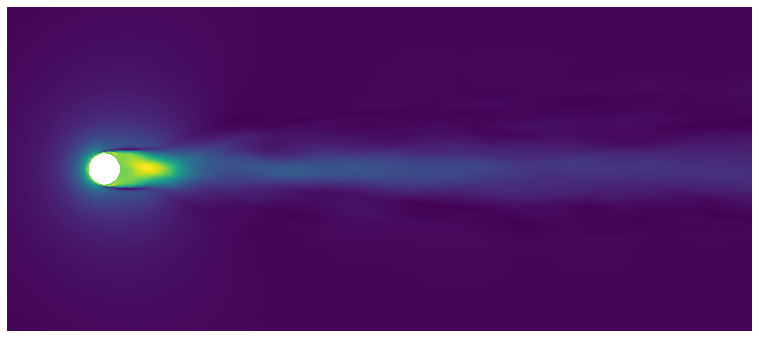
\includegraphics[width=0.49\textwidth]{figs/cyl_2580_0}
    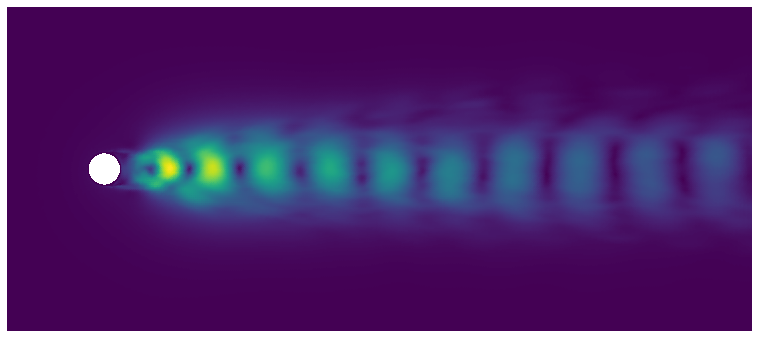
\includegraphics[width=0.49\textwidth]{figs/cyl_2580_1} \\
    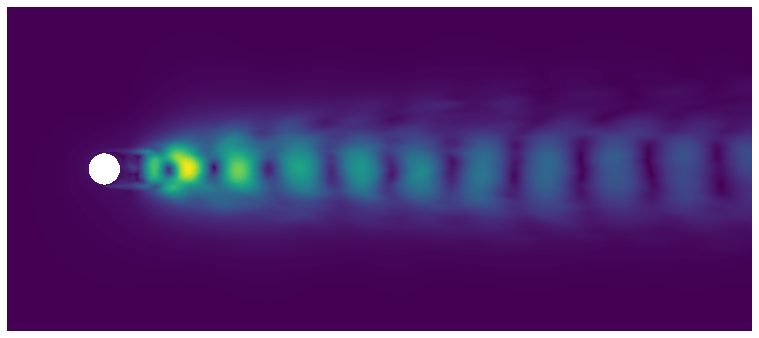
\includegraphics[width=0.49\textwidth]{figs/cyl_2580_2}
    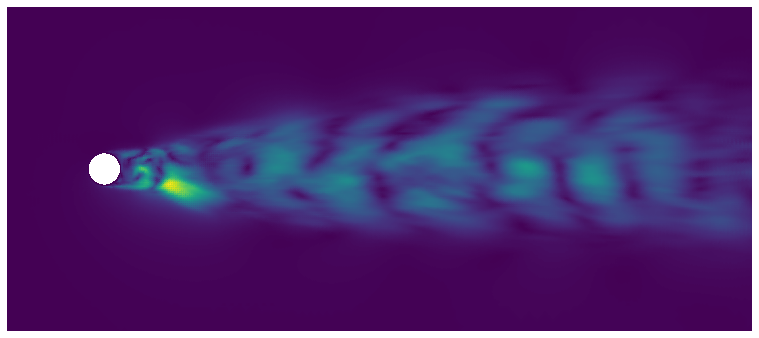
\includegraphics[width=0.49\textwidth]{figs/cyl_2580_3}
  \end{center}
\end{frame}

\begin{frame}[fragile]
  \frametitle{Cylinder, $\text{Re}=2580$, spectrum (normalized)}

  \begin{center}
    \begin{tikzpicture}
      \begin{axis}[
        ymode=log,
        grid=both,
        legend cell align=left,
        xmin=1, xmax=200,
        ]
        \addplot[magenta, very thick]
        table[x index={0}, y index={1}]{data/cyl_2580.csv};
        \addplot[blue, very thick]
        table[x index={0}, y index={2}]{data/cyl_2580.csv};
        \addplot[red, very thick]
        table[x index={0}, y index={3}]{data/cyl_2580.csv};
        \legend{
          $\lambda_k$,
          Energy tail,
          Error,
        }
      \end{axis}
    \end{tikzpicture}
  \end{center}
\end{frame}

\begin{frame}[fragile]
  \frametitle{Cylinder, $\text{Re}=40000$, first four modes}

  \begin{center}
    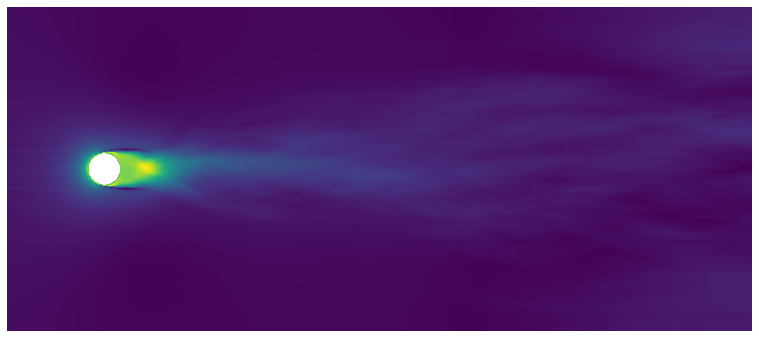
\includegraphics[width=0.49\textwidth]{figs/cyl_40k_0}
    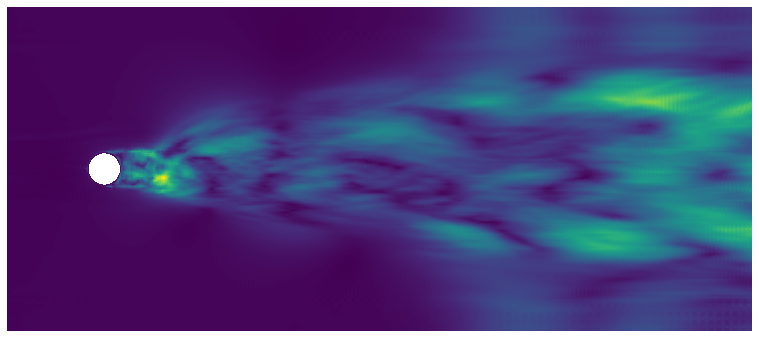
\includegraphics[width=0.49\textwidth]{figs/cyl_40k_1} \\
    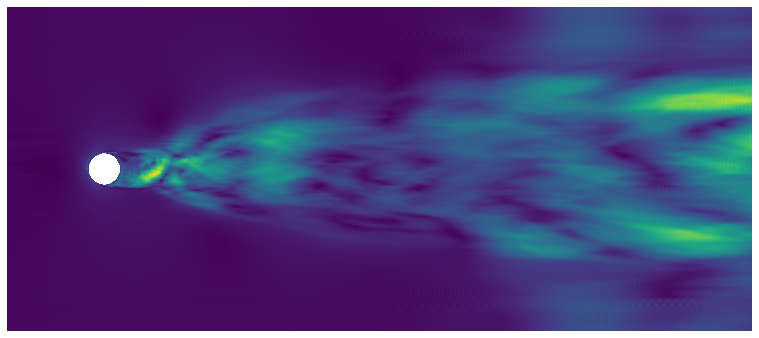
\includegraphics[width=0.49\textwidth]{figs/cyl_40k_2}
    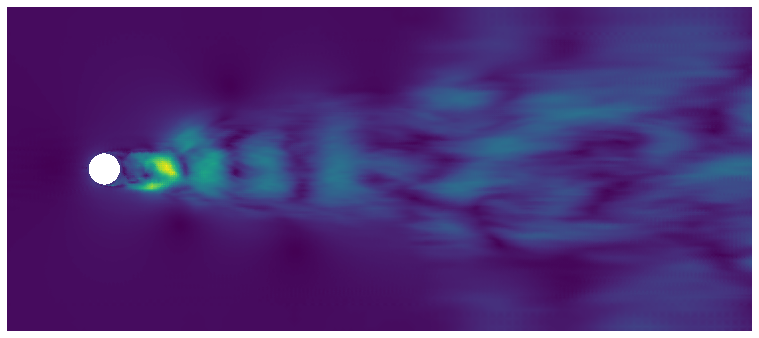
\includegraphics[width=0.49\textwidth]{figs/cyl_40k_3}
  \end{center}
\end{frame}

\begin{frame}[fragile]
  \frametitle{Cylinder, $\text{Re}=40000$, spectrum (normalized)}

  \begin{center}
    \begin{tikzpicture}
      \begin{axis}[
        ymode=log,
        grid=both,
        legend cell align=left,
        xmin=1, xmax=200,
        ]
        \addplot[magenta, very thick]
        table[x index={0}, y index={1}]{data/cyl_40k.csv};
        \addplot[blue, very thick]
        table[x index={0}, y index={2}]{data/cyl_40k.csv};
        \addplot[red, very thick]
        table[x index={0}, y index={3}]{data/cyl_40k.csv};
        \legend{
          $\lambda_k$,
          Energy tail,
          Error,
        }
      \end{axis}
    \end{tikzpicture}
  \end{center}
\end{frame}

\begin{frame}[fragile]
  \frametitle{NACA 0015, $\text{Re}=2\times\SI{e3}{}$, first four mode}

  \begin{center}
    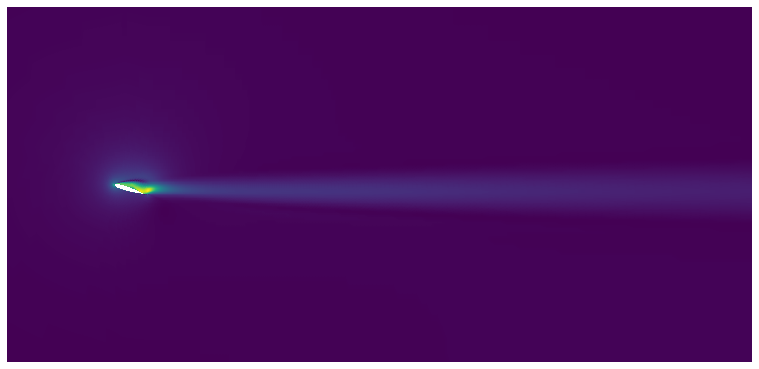
\includegraphics[width=0.49\textwidth]{figs/naca4_0}
    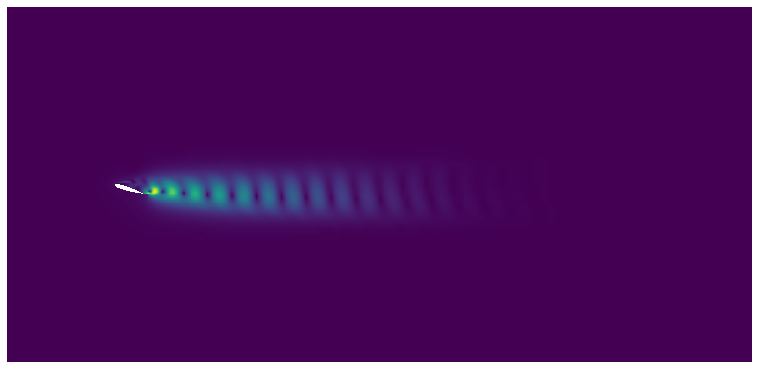
\includegraphics[width=0.49\textwidth]{figs/naca4_1} \\
    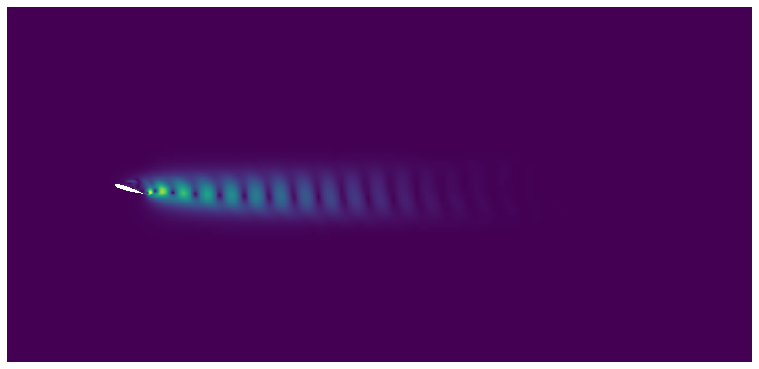
\includegraphics[width=0.49\textwidth]{figs/naca4_2}
    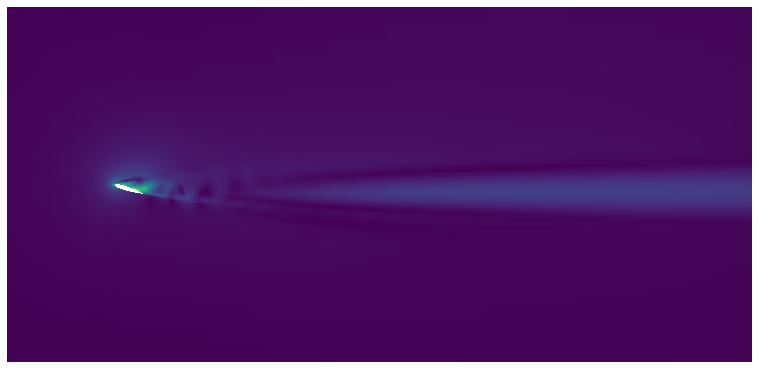
\includegraphics[width=0.49\textwidth]{figs/naca4_3}
  \end{center}
\end{frame}

\begin{frame}[fragile]
  \frametitle{NACA 0015, $\text{Re}=2\times\SI{e3}{}$, spectrum (normalized)}

  \begin{center}
    \begin{tikzpicture}
      \begin{axis}[
        ymode=log,
        grid=both,
        legend cell align=left,
        xmin=1, xmax=200,
        ]
        \addplot[magenta, very thick]
        table[x index={0}, y index={1}]{data/naca4.csv};
        \addplot[blue, very thick]
        table[x index={0}, y index={2}]{data/naca4.csv};
        \addplot[red, very thick]
        table[x index={0}, y index={3}]{data/naca4.csv};
        \legend{
          $\lambda_k$,
          Energy tail,
          Error,
        }
      \end{axis}
    \end{tikzpicture}
  \end{center}
\end{frame}

\begin{frame}[fragile]
  \frametitle{NACA 0015, $\text{Re}=2\times\SI{e4}{}$, first four mode}

  \begin{center}
    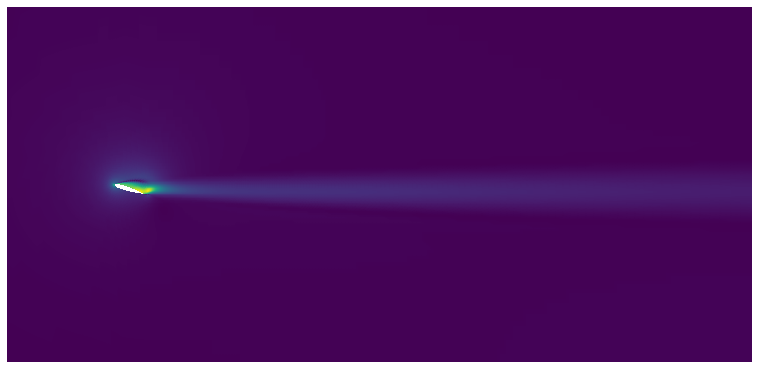
\includegraphics[width=0.49\textwidth]{figs/naca5_0}
    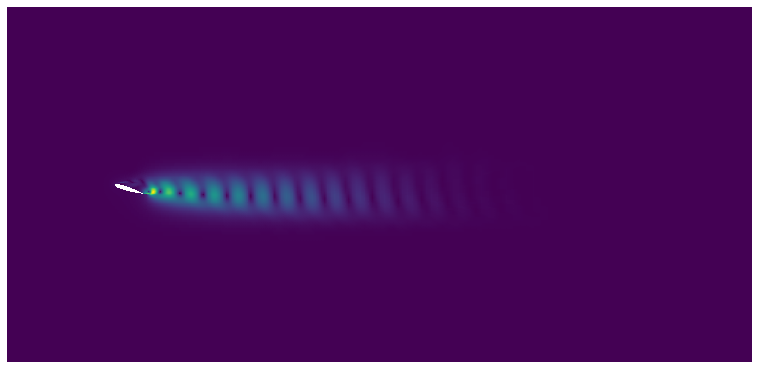
\includegraphics[width=0.49\textwidth]{figs/naca5_1} \\
    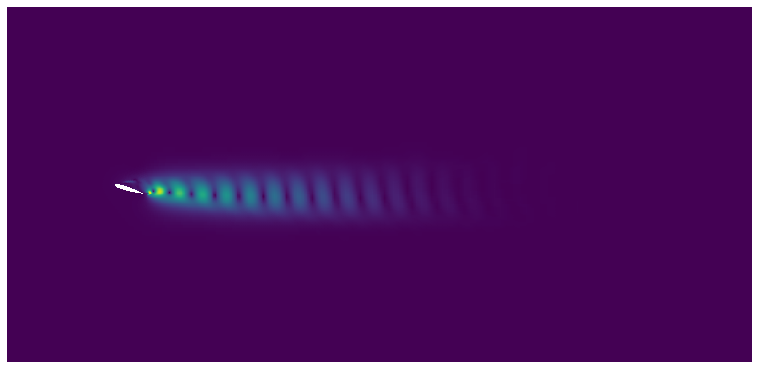
\includegraphics[width=0.49\textwidth]{figs/naca5_2}
    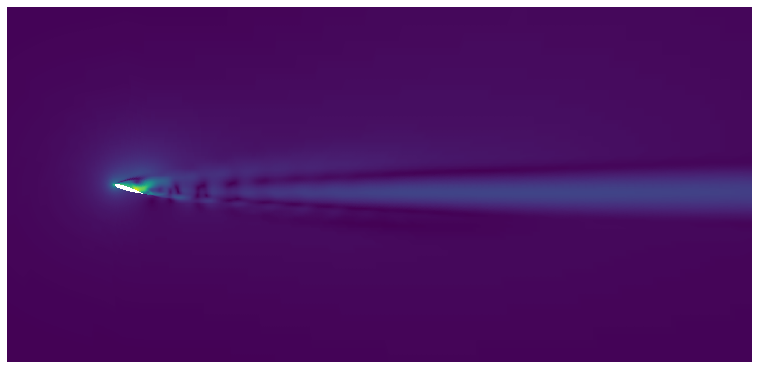
\includegraphics[width=0.49\textwidth]{figs/naca5_3}
  \end{center}
\end{frame}

\begin{frame}[fragile]
  \frametitle{NACA 0015, $\text{Re}=2\times\SI{e4}{}$, spectrum (normalized)}

  \begin{center}
    \begin{tikzpicture}
      \begin{axis}[
        ymode=log,
        grid=both,
        legend cell align=left,
        xmin=1, xmax=200,
        ]
        \addplot[magenta, very thick]
        table[x index={0}, y index={1}]{data/naca5.csv};
        \addplot[blue, very thick]
        table[x index={0}, y index={2}]{data/naca5.csv};
        \addplot[red, very thick]
        table[x index={0}, y index={3}]{data/naca5.csv};
        \legend{
          $\lambda_k$,
          Energy tail,
          Error,
        }
      \end{axis}
    \end{tikzpicture}
  \end{center}
\end{frame}

\begin{frame}[fragile]
  \frametitle{NACA 0015, $\text{Re}=2\times\SI{e5}{}$, first mode}

  \begin{center}
    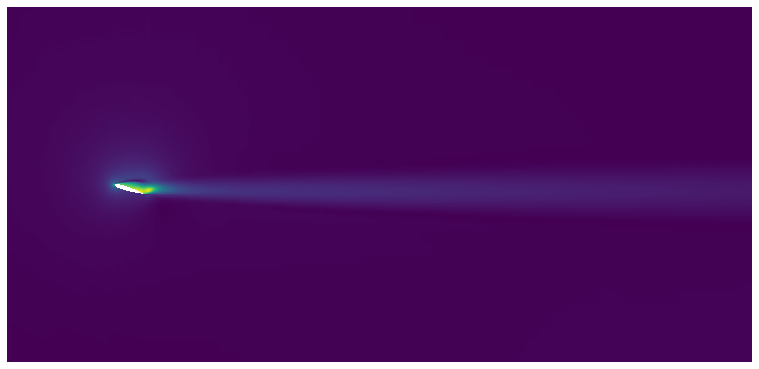
\includegraphics[width=0.49\textwidth]{figs/naca6_0}
    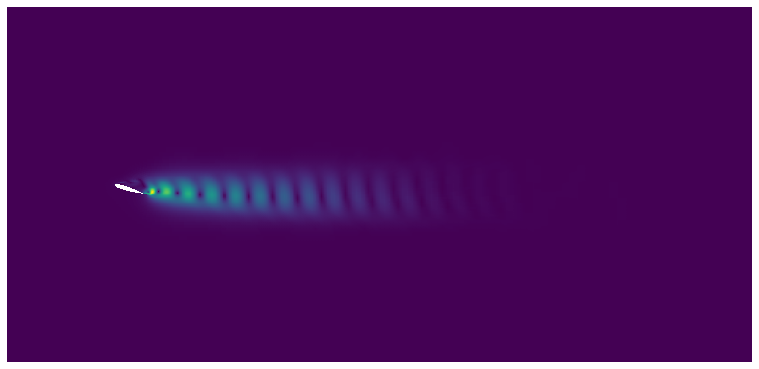
\includegraphics[width=0.49\textwidth]{figs/naca6_1} \\
    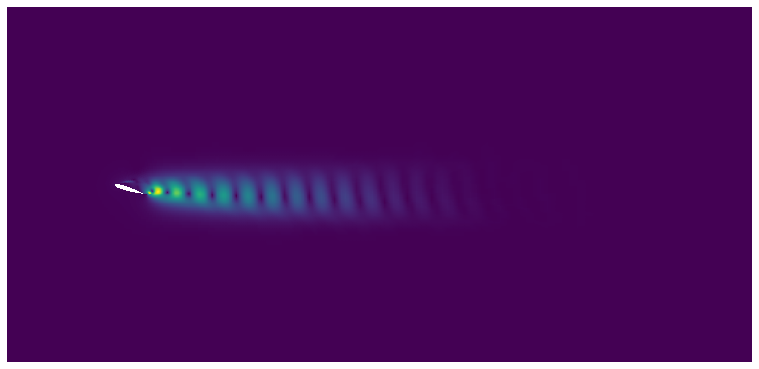
\includegraphics[width=0.49\textwidth]{figs/naca6_2}
    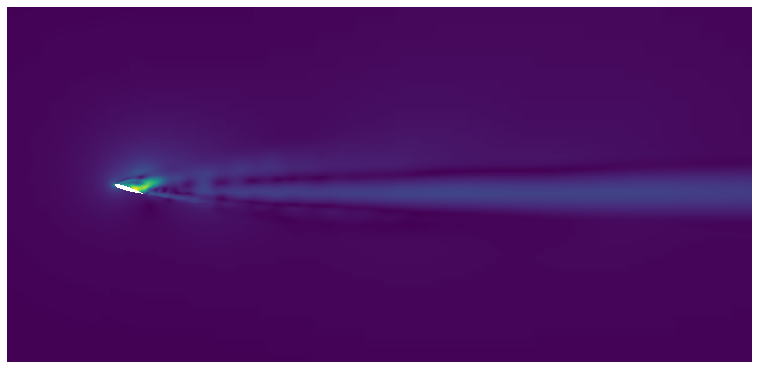
\includegraphics[width=0.49\textwidth]{figs/naca6_3}
  \end{center}
\end{frame}

\begin{frame}[fragile]
  \frametitle{NACA 0015, $\text{Re}=2\times\SI{e5}{}$, spectrum (normalized)}

  \begin{center}
    \begin{tikzpicture}
      \begin{axis}[
        ymode=log,
        grid=both,
        legend cell align=left,
        xmin=1, xmax=200,
        ]
        \addplot[magenta, very thick]
        table[x index={0}, y index={1}]{data/naca6.csv};
        \addplot[blue, very thick]
        table[x index={0}, y index={2}]{data/naca6.csv};
        \addplot[red, very thick]
        table[x index={0}, y index={3}]{data/naca6.csv};
        \legend{
          $\lambda_k$,
          Energy tail,
          Error,
        }
      \end{axis}
    \end{tikzpicture}
  \end{center}
\end{frame}

\begin{frame}[fragile]
  \frametitle{Conclusions}

  \begin{itemize}
  \item For a large variety of flow problems, a few hundred degrees of freedom
    suffice for mean relative \emph{approximation errors} of $\SI{e-2}{}$ to
    $\SI{e-5}{}$ depending on circumstances.
  \item Encouraging preliminary results that promise potentially fast flow
    solvers for repetitive applications with ``practical'' error requirements.
  \end{itemize}
\end{frame}

\end{document}
